\documentclass{article}
\title{CS 551 Project 1 Report}
\author{Group 20 \\\\ Ryan Attard, Sean Wallace,Velin Sedlarski,Adrian Birylo\\\\}
\date{October 25, 2013}

\usepackage{fullpage}
\usepackage{enumerate}

\usepackage{graphicx}

\usepackage{fancyvrb}
\DefineVerbatimEnvironment{code}{Verbatim}{fontsize=\small}
\DefineVerbatimEnvironment{example}{Verbatim}{fontsize=\small}
\newcommand{\ignore}[1]{}

\usepackage[usenames]{color}
\usepackage{listings}
\lstset{ %
	language=bash,                			% choose the language of the code
	basicstyle=\footnotesize,       			% the size of the fonts that are used for the code
	numbers=left,                   			% where to put the line-numbers
	numberstyle=\footnotesize,				% the size of the fonts that are used for the line-numbers
	stepnumber=1,                   			% the step between two line-numbers. If it is 1 each line will be numbered
	numbersep=5pt,                  			% how far the line-numbers are from the code
	backgroundcolor=\color{white},			% choose the background color. You must add \usepackage{color}
	showspaces=false,               			% show spaces adding particular underscores
	showstringspaces=false,         			% underline spaces within strings
	showtabs=false,                 			% show tabs within strings adding particular underscores
	frame=single,                   			% adds a frame around the code
	tabsize=2,              					% sets default tabsize to 2 spaces
	captionpos=t,	                   		% sets the caption-position to bottom
	breaklines=true,        					% sets automatic line breaking
	breakatwhitespace=false,    				% sets if automatic breaks should only happen at whitespace
	escapeinside={\%}{)}          			% if you want to add a comment within your code
}

\begin{document}
\maketitle
\pagebreak 
\section{API}

\subsection{int IGInit()}
This function initializes the messaging system. It resets all of the buffers and counters. Only one process should call IGInit since subsequent calls to IGInit will remove any data that may be in the buffer by previous processes. This function will always return 1. 

\subsection{int IGLookup(int groupID)}
This function looks up if there is an interest group with the specified groupID and returns 1 if the groupID exists or 0 if it doesn't exist.

\subsection{int IGCreate(int groupID)}
This function creates an interest group with the specified groupID and returns with 1. If the groupID already exist then no interest group is created and returns with 0. 

\subsection{int IGPublisher(int callerID, int groupID)}
This function registers the callerID with the specified groupID as a publisher if the groupID exists and the max amount of registered publishers/subscribers is not reached and return 1 on success. If the interest groupID doesn't exist or the max amount of registered publishers/subscribers are reach then the publisher is not registered and returns with 0.

\subsection{int IGSubscriber(int callerID, int groupID)}
This function registers the callerID with the specified groupID as a subscriber if the groupID exists and the max amount of registered publishers/subscribers is not reached and return 1 on success. If the interest groupID doesn't exist or the max amount of registered publishers/subscribers are reach then the subscriber is not registered and returns with 0.

\subsection{int IGPublish(int callerID, int groupID, int message)}
This function publishes the message if the groupID is registered and the callerID is registered as a publisher to the groupID and the function returns 1. If the buffer is full then the function returns 0. Also if the callerID is not part of the groupID or a publisher to the groupID it will not publish the message and return 0.

\subsection{int IGRetrieve(int callerID, int groupID, int message)}
This function retrieves the message if the groupID is registered and the callerID is registered as a subscriber to the groupID and the function returns a positive number which is the message. If there are no messages in the buffer then the function return -1. Also if the callerID is not part of the groupID or a subscribe to the groupID it will not retrieve the message and return -1.


\section{Design}
The design of the IPC system call is such that it was added to the Process Management (PM) service. Below is a block diagram of how the IPC is implemented and what is in the user space and what is a service and in the kernel space. 

\begin{figure}[!h]
\center{
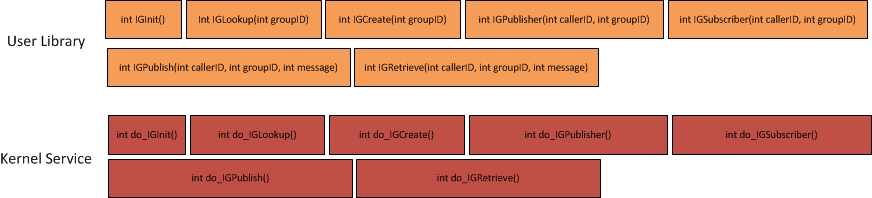
\includegraphics[width=\textwidth]{FlowChart.png}
\caption{Flow Chart}
}
\end{figure}

\section{Discussion}
In general deadlock can not occur since there are no blocking calls but a poorly written program can go into deadlock. Since there is no blocking calls a process is never waiting to get or put data in the IPC. Since the calls are not blocking they can fail and it is the responsibility of the programmer to make sure to recover from a failure gracefully and retry. 



\end{document}
